% This file was created with tikzplotlib v0.10.1.
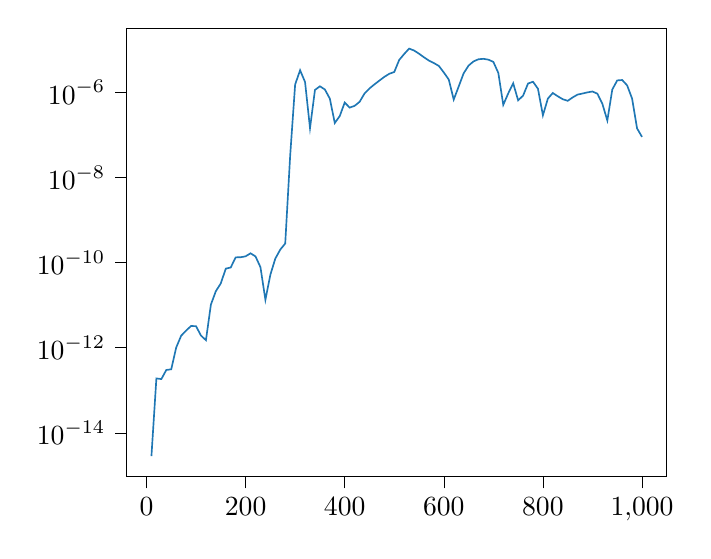
\begin{tikzpicture}

\definecolor{darkgray176}{RGB}{176,176,176}
\definecolor{steelblue31119180}{RGB}{31,119,180}

\begin{axis}[
log basis y={10},
tick align=outside,
tick pos=left,
x grid style={darkgray176},
xmin=-39.5, xmax=1049.5,
xtick style={color=black},
y grid style={darkgray176},
ymin=9.39860275109877e-16, ymax=3.22537233538702e-05,
ymode=log,
ytick style={color=black},
ytick={1e-18,1e-16,1e-14,1e-12,1e-10,1e-08,1e-06,0.0001,0.01},
yticklabels={
  \(\displaystyle {10^{-18}}\),
  \(\displaystyle {10^{-16}}\),
  \(\displaystyle {10^{-14}}\),
  \(\displaystyle {10^{-12}}\),
  \(\displaystyle {10^{-10}}\),
  \(\displaystyle {10^{-8}}\),
  \(\displaystyle {10^{-6}}\),
  \(\displaystyle {10^{-4}}\),
  \(\displaystyle {10^{-2}}\)
}
]
\addplot [semithick, steelblue31119180]
table {%
10 2.83106871279415e-15
20 1.90347737571983e-13
30 1.83686399424232e-13
40 3.00037772404949e-13
50 3.12361247978288e-13
60 1.01413322184385e-12
70 1.91702209662026e-12
80 2.53269627492614e-12
90 3.24912319271675e-12
100 3.20993231994748e-12
110 1.9320101074527e-12
120 1.50446322066955e-12
130 1.03387853833681e-11
140 2.13758455380741e-11
150 3.25320881344737e-11
160 7.23269777402891e-11
170 7.69216357277003e-11
180 1.33128286172735e-10
190 1.33857036566098e-10
200 1.40736089448978e-10
210 1.65848335065277e-10
220 1.40078060262283e-10
230 7.83835218953755e-11
240 1.33861255413592e-11
250 5.20516407753746e-11
260 1.24548094060373e-10
270 2.02686367689608e-10
280 2.81527468004583e-10
290 3.31093481520384e-08
300 1.53599114582903e-06
310 3.3221888315893e-06
320 1.75943387148436e-06
330 1.44632409160295e-07
340 1.14183296773263e-06
350 1.39451469749474e-06
360 1.1723386705853e-06
370 7.16215993179503e-07
380 1.9117548788472e-07
390 2.78085906302294e-07
400 5.78075685098156e-07
410 4.39809923591383e-07
420 4.83714472920838e-07
430 5.99557665736938e-07
440 9.41520397645945e-07
450 1.23993675060774e-06
460 1.54450640366122e-06
470 1.897102492876e-06
480 2.31704257203091e-06
490 2.74648164122482e-06
500 3.01858176499081e-06
510 5.79840616410365e-06
520 7.9871033449308e-06
530 1.07076148196938e-05
540 9.66580137173878e-06
550 8.12423877505353e-06
560 6.69581686452148e-06
570 5.59806403543917e-06
580 4.90427191834897e-06
590 4.18978288507788e-06
600 2.94750338980521e-06
610 2.01242505681876e-06
620 6.7872974796046e-07
630 1.37247013753949e-06
640 2.80694257526193e-06
650 4.27310897066491e-06
660 5.36211973667378e-06
670 6.01785086473683e-06
680 6.16137049291865e-06
690 5.88616239838302e-06
700 5.21771471539978e-06
710 2.87883813143708e-06
720 5.10911377205048e-07
730 9.47674379858654e-07
740 1.64145990311226e-06
750 6.52616677143669e-07
760 8.40697964576975e-07
770 1.62052003815916e-06
780 1.7824141878009e-06
790 1.22035839922319e-06
800 2.90055993446003e-07
810 7.15911369297828e-07
820 9.70316250459291e-07
830 8.12172231690056e-07
840 6.92953790348838e-07
850 6.33950037354225e-07
860 7.6307139806886e-07
870 8.90032083589176e-07
880 9.42112137636286e-07
890 1.00397846836131e-06
900 1.05163940133934e-06
910 9.33167427774606e-07
920 5.39498444140918e-07
930 2.18982165733905e-07
940 1.17058334581088e-06
950 1.91785420611268e-06
960 1.95658822121914e-06
970 1.46171657888772e-06
980 7.14970553872263e-07
990 1.42909087230692e-07
1000 9.00235974654606e-08
};
\end{axis}

\end{tikzpicture}
